\section{Solution Design and Implementation}
\label{sec:parallelization}

To harness the speedups offered by parallel computing, we used the OpenMPI library.
The first step was to choose which part of the program to parallelize.
This has been easy: the recursive part.
the points are divided among the processes, then merged.
It was now time to decide how to communicate amongst processes, and we came up with the scheme of which in \Cref{fig:albero_bell_albero}.
The splitting of the work can be visualized as a tree, in which each node does the same amount of work. The nodes on the left communicate to the nodes on the right.

\begin{figure}[!ht]
  \resizebox{\columnwidth}{!}{
    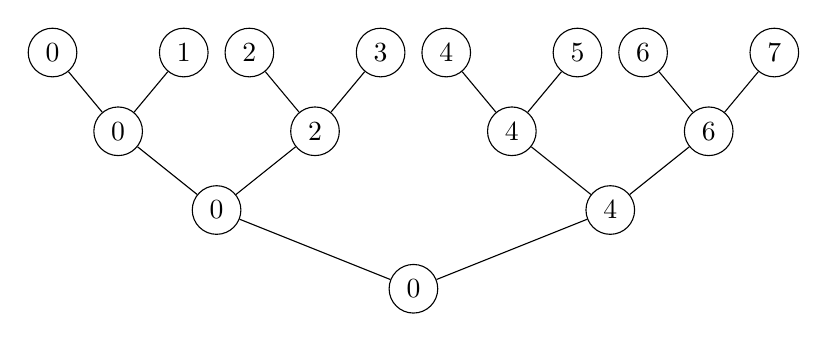
\begin{tikzpicture}[
        grow'=up,
        every node={
                style={
                        draw,align=center
                    }
            },
        level distance=1cm,
        level/.style={sibling distance=5cm/#1}
    ]
    \tikzset  {
        treenode/.style = {circle, draw=black, align=center, minimum size=0.5cm},
    }
    \node [treenode] {0}
    child {
            node [treenode] {0}
            child
                {
                    node [treenode] {0}
                    child {
                            node [treenode] {0}
                        }
                    child {
                            node [treenode] {1}
                        }
                }
            child
                {
                    node [treenode] {2}
                    child {
                            node [treenode] {2}
                        }
                    child {
                            node [treenode] {3}
                        }
                }
        }
    child {
            node [treenode] {4}
            child
                {
                    node [treenode] {4}
                    child {
                            node [treenode] {4}
                        }
                    child {
                            node [treenode] {5}
                        }
                }
            child
                {
                    node [treenode] {6}
                    child {
                            node [treenode] {6}
                        }
                    child {
                            node [treenode] {7}
                        }
                }
        }
    ;
\end{tikzpicture}

  }
  \caption{Illustration of the process communication scheme with 8 processes.}
  \label{fig:albero_bell_albero}
\end{figure}

It was now time to implement it with OpenMPI. This required several modifications to the code. The first thing was to decide which MPI calls to make.
Process 0 is the one that reads the file initially and then reassembles the final result.
The natural choice at the beginning to distribute the points was a \verb+MPI_Scatterv+. To do this we had to implement two MPI datatypes, \verb+mpi_point_type+ to represent a point and \verb+mpi_pair_of_points_type+
to represent a pair of points.
Then each process receives its points and can work on them. Each process knows how many points to receive since they received the total count of points from 0 with a broadcast.
After the process computed its closest pair, it calculates the bands according to the smallest distance it found and sends them to the receiving process.
This would call for four MPI send operations (left band count, right band count, left band points, right band points). Instead, we optimized this by sending the two lengths simultaneously and then the concatenation of the band points.
